\documentclass[a4paper, 12pt]{article}

\usepackage[portuges]{babel}
\usepackage[utf8]{inputenc}
\usepackage{amsmath}
\usepackage{indentfirst}
\usepackage{blindtext}
\usepackage{graphicx}
\usepackage[hidelinks]{hyperref}
\usepackage{gensymb}
\usepackage{pgfplots}

\author{Igor Abreu da Silva}

\title{Lista Sistemas Lineares I}

\begin{document}

    \begin{titlepage}
        \begin{center}
            \huge{Universidade Federal do Rio de Janeiro}
            \vspace{95pt}

            \large{Lista II - Sistemas Lineares I}
            \vspace{160pt}
        \end{center}

        \begin{flushleft}
            \begin{tabbing}
                Alunos\qquad\qquad\= Igor Abreu da Silva\\
                DRE\> 112053874 \\
                Curso\> Engenharia Eletrônica \\
                Turma\> 2016/2 \\
                Professor\> Natanael Nunes de Moura Junior \\

            \end{tabbing}

        \end{flushleft}

        \begin{center}
            \vspace{\fill}
            Rio de Janeiro, 04 de Outubro de 2016
        \end{center}
    \end{titlepage}

    \newpage
    \tableofcontents
    \listoffigures
    \thispagestyle{empty}
    \newpage
    \pagenumbering{arabic}
    
    \section{An\'{a}lise de Sistema no Dom\'{i}nio do Tempo}
    \subsection{Quest\~{a}o 1}
    \subsubsection{Item a}
    \[\lambda^{2} + 5\lambda + 6 = 0 \rightarrow \lambda_{1} = -2; \lambda_{2} = -3 \rightarrow c_{1}e^{-2t} + c_{2}e^{-3t}\]
    \subsubsection{Item b}
    \[c_{1} + c_{2} = 2 \]
    \[-2c_{1} -3c_{2} = -1 \]
    \[c_{1} =  5\]
    \[c_{2} =  -3\]    
    \[y_{0} = 5e^{-2t} -3e^{-3t} \]
    \subsection{Quest\~{a}o 2}
    \subsubsection{Item a}   
    \[ \lambda^{2} + \lambda = 0 \rightarrow  \lambda_{1} = 0; \lambda_{2} = -1 \rightarrow c_{1}^{-2+3j} +c_{2}e^{-t}\]   
    \subsubsection{Item b}
    \[c_{1} + c_{2} = 1 \]
    \[-c_{2} = 1 \]
    \[c_{1} =  2\]
    \[c_{2} =  -1\]    
    \[y_{0} = 2 -e^{-t} \]    
    \subsection{Quest\~{a}o 3}
    \subsubsection{Item a}   
    \[\lambda^{2} + 4\lambda + 13 = 0 \rightarrow  \lambda_{1} = -2 + 3j; \lambda_{2} = -2 -3j \rightarrow c_{1}e^{(-2+3j)t} +c_{2}e^{(-2-3j)t} = ce^{-2t}cos(3t + \phi)\]   
    \subsubsection{Item b}
    \[ccos(\phi) = 1 \]
    \[-2ccos(\phi) -3csen(\phi) = 15.98 \]
    \[c =  10\]
    \[\phi =  \frac{-\pi}{3}\]    
    \[y_{0} = 10e^{-2t}cos(3t - \frac{\pi}{3}) \]      
    \subsection{Quest\~{a}o 4}
    \subsubsection{Item a}   
    \[ (\lambda + 1)(\lambda^{2} + 5\lambda + 6) = 0 \rightarrow  \lambda_{1} = -1; \lambda_{2} = -2; \lambda_{3} = -3 \rightarrow c_{1}e^{-t} +c_{2}e^{-2t} + c_{3}e^{-3t}\]   
    \subsubsection{Item b}
    \[c_{1} + c_{2} + c_{3}  = 2 \]
    \[-c_{1} -2c_{2} -3c_{3} = -1 \]
    \[c_{1} +4c_{2} +9c_{3} =  5\]
    \[c_{1} =  6\]    
    \[c_{2} =  -7\]
    \[c_{3} =  3\]
    \[y_{0} =  6e^{-t} -7e^{-2t} + 3e^{-3t}\]   
    \subsection{Quest\~{a}o 5}
    \[A_{c} = \int_{-\infty}^{\infty} c(t)\]
    \[c(t) = \int_{-\infty}^{\infty} x(\tau)g(t -\tau)d\tau\]
    \[A_{c} = \int_{-\infty}^{\infty} [\int_{-\infty}^{\infty} x(\tau)g(t -\tau)d\tau] dt \rightarrow \int_{-\infty}^{\infty} [\int_{-\infty}^{\infty} x(\tau)d\tau][g(t -\tau)] dt \Rightarrow\]
    \[\int_{-\infty}^{\infty} A_{x}[g(t -\tau)] dt = A_{x}\int_{-\infty}^{\infty}g(t -\tau)dt = A_{x}A_{g} \]
    
    \subsection{Quest\~{a}o 6}
    \[c(t) = x(t)\ast g(t) \rightarrow \int_{-\infty}^{\infty} x(\tau)g(t -\tau)d\tau\]
    \[c(at) = x(at)\ast g(at) \rightarrow \int_{-\infty}^{\infty} x(a\tau)g(a[t - \tau])d\tau \rightarrow \frac{1}{a}\int_{-\infty}^{\infty} x(w)g(at - w)dw = \frac{c(at)}{a}\]
    \subsection{Quest\~{a}o 7} 
    \[y(t) = x_{par}(t)\ast g_{impar}(t) \rightarrow \int_{-\infty}^{\infty} x(\tau)g(t -\tau)d\tau \Rightarrow\]
    \[\int_{-\infty}^{\infty} \frac{[x(\tau) + x(-\tau)]}{2}\frac{g(t -\tau) - g(\tau - t)}{2}d\tau\]    
    Travei
    \subsection{Quest\~{a}o 8}
    \[ e^{-at}u(t)\ast e^{-bt}u(t) \rightarrow \int_{0}^{\infty} e^{-a\tau}e^{-b(t-\tau)}d\tau \rightarrow \int_{0}^{\infty} e^{-a\tau}e^{-bt}e^{b\tau}d\tau \rightarrow e^{-bt}\int_{0}^{\infty} e^{-\tau(a-b)}d\tau \Rightarrow\]
    \[ e^{-bt}[\frac{-1}{a-b}] = \frac{-e^{-bt}}{a-b}u(t)\]
    \subsection{Quest\~{a}o 9}
    \[ \int_{-\infty}^{+\infty} sin(\tau)u(t-\tau) d\tau \rightarrow \int_{0}^{t} sin(\tau) d\tau = (-cos(t) + 1)u(t)\]    
    \[ \int_{-\infty}^{+\infty} cos(\tau)u(t-\tau) d\tau \rightarrow \int_{0}^{t} cos(\tau) d\tau = sen(t)u(t)\]       
    \subsection{Quest\~{a}o 10}
    \subsubsection{Item a} 
    \[ \int_{-\infty}^{+\infty} e^{-\tau}u(t)u(t-\tau) d\tau \rightarrow \int_{0}^{t} e^{-\tau} d\tau = (-e^{-t} + 1)u(t)\]        
    \subsubsection{Item b} 
    \[ \int_{-\infty}^{+\infty} e^{-\tau}u(t)e^{-(t-\tau)}u(t) d\tau \rightarrow \int_{0}^{t} e^{-\tau}e^{-(t-\tau)} d\tau = e^{-t}\int_{0}^{t} d\tau = te^{-t}\]       
    \subsubsection{Item c} 
    \[ \int_{-\infty}^{+\infty} e^{-\tau}u(t)e^{-2(t-\tau)}u(t) d\tau \rightarrow \int_{0}^{t} e^{-\tau}e^{-2(t-\tau)} d\tau \rightarrow e^{-2t}\int_{0}^{t} e^{\tau}d\tau = e^{-2t}(e^{t} -1)\]          
    \subsubsection{Item d} 
    \[ \int_{-\infty}^{+\infty} e^{-\tau}u(t)sin(3(t-\tau))u(t) d\tau \rightarrow \int_{0}^{t} e^{-\tau}sin(3t-3\tau) d\tau = \frac{3e^{-t}+sin(3t)-3cos(3t)}{10}\]       
    \subsection{Quest\~{a}o 11}
    \subsubsection{Item a} 
    \[ \int_{-\infty}^{+\infty} e^{-\tau}u(t)[-\delta(t-\tau) + 2e^{-(t-\tau)}]u(t) d\tau \rightarrow \int_{0}^{+\infty} e^{-\tau}-\delta(t-\tau)d\tau + \int_{0}^{t}e^{-\tau}2e^{-(t-\tau)}d\tau \Rightarrow\]     
    \[-e^{-t} + 2te^{-t}\]
    \newpage
    \subsubsection{Item b} 
    \begin{figure}[!ht]
          	\centering
          	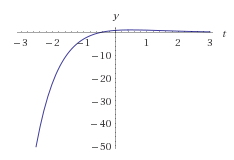
\includegraphics{img/Figura1.PNG}
          	\caption{Resposta ao Estado Nulo - Quest\~{a}o 11}
    \end{figure}    
    
    \subsection{Quest\~{a}o 12}
    \begin{figure}[!ht]
    	\centering
    	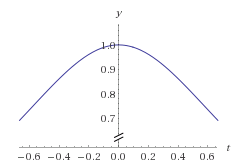
\includegraphics{img/Figura2.PNG}
    	\caption{Sinal $\frac{1}{t^{2} + 1}$}
    \end{figure}       
    \begin{figure}[!ht]
    	\centering
    	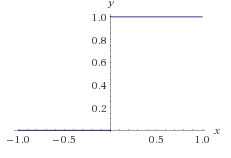
\includegraphics{img/Figura3.PNG}
    	\caption{Sinal Degrau}
    \end{figure}           
    \[ \int_{-\infty}^{+\infty} \frac{1}{\tau^{2} + 1}u(t) d\tau \rightarrow \int_{0}^{+\infty} \frac{1}{\tau^{2} + 1} = arctg(t) + \frac{\pi}{2}\]     
    \begin{figure}[!ht]
    	\centering
    	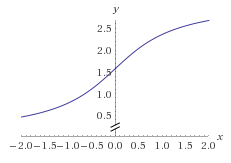
\includegraphics{img/Figura4.PNG}
    	\caption{Convolução dos sinais}
    \end{figure}        
    \subsection{Quest\~{a}o 13}
        \begin{tikzpicture}
        \begin{axis}[%
        ,xlabel=$t$
        ,ylabel=$u(t)$
        ,axis x line = bottom,axis y line = left
        ,ytick={1,2,3,4}
        ,ymax=4 % or enlarge y limits=upper
        ]
        \addplot+[const plot, no marks, thick,blue] coordinates {(0,0) (1,0) (2,0)} {};                
        \addplot[domain=2:3,blue]{x-2};
        \addplot+[const plot, no marks, thick,blue] coordinates {(3,1) (4,1) (5,1) (6,1) (7,1) (8,1)} {};
        \addplot[domain=8:9,blue]{-x+9};
        \end{axis}
        \end{tikzpicture}    
    \subsection{Quest\~{a}o 14}
    \[ \int_{-\infty}^{+\infty} sin(\tau)u(t - \tau) d\tau \rightarrow \int_{0}^{t} sin(\tau) d\tau = 1 - cos(t)\]      
    \begin{figure}[!ht]
    	\centering
    	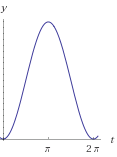
\includegraphics{img/Figura5.PNG}
    	\caption{$sin(t) \ast u(t)$}
    \end{figure}                  
    \subsection{Quest\~{a}o 15}
    \subsubsection{Item a} 
        \begin{tikzpicture}
        \begin{axis}[%
        ,xlabel=$t$
        ,ylabel=$u(t)$
        ,axis x line = bottom,axis y line = left
        ,ytick={1,2}
        ,ymax=2 % or enlarge y limits=upper
        ]             
        \addplot[domain=0:1,blue]{1-x};
        \end{axis}
        \end{tikzpicture}
         
        \begin{tikzpicture}
        \begin{axis}[%
        ,xlabel=$t$
        ,ylabel=$u(t)$
        ,axis x line = bottom,axis y line = left
        ,ytick={-2,-1,0,1,2,3}
        ,ymax=3 % or enlarge y limits=upper
        ]             
        \addplot[domain=-2:2,blue]{x};
        \addplot+[const plot, no marks, thick,blue] coordinates {(2,2) (2,0) (3,0)}{};
        \end{axis}
        \end{tikzpicture}           
    \subsubsection{Item b} 
        \begin{tikzpicture}
        \begin{axis}[%
        ,xlabel=$t$
        ,ylabel=$u(t)$
        ,axis x line = bottom,axis y line = left
        ,ytick={-2,-1,0,1,2,3}
        ,ymax=3 % or enlarge y limits=upper
        ]             
        \addplot[domain=-2:0,blue]{x};
        \addplot+[const plot, no marks, thick,blue] coordinates {(0,0) (0,1) (1,1)} {};        
        \addplot[domain=1:2,blue]{x};
        \addplot+[const plot, no marks, thick,blue] coordinates {(2,2) (2,0) (3,0)}{};
        \end{axis}
        \end{tikzpicture}        
    \subsubsection{Item c}     
	Não consegui fazer
    \subsection{Quest\~{a}o 16}
    Não consegui fazer
    \section{An\'{a}lise de Sistema no Dom\'{i}nio Laplace}      
    \subsection{Quest\~{a}o 1}
    \subsubsection{Item a} 
    \[\int_{0}^{1} e^{-st}dt = \frac{(1-e^{-s})}{s} \]
    \subsubsection{Item b} 
    \[\int_{0}^{\infty} te^{-t}e^{-st}dt = \int_{0}^{\infty} te^{-t(s+1)}dt = \frac{1}{(s+1)^{2}}\]
    \subsubsection{Item c} 
    \[\int_{0}^{\infty} tcos(w_{0}t)e^{-st}dt = \frac{1}{2}\int_{0}^{\infty}(e^{jw_{0}t} + e^{-jw_{0}t})te^{-st}dt = \frac{1}{(s+1)^{2}} \Rightarrow\]
    \[\frac{1}{2}\int_{0}^{\infty}(te^{t(s-jw_{0})} + te^{t(s+jw_{0})})dt = \frac{1}{2(s-jw_{0})^{2}} +\frac{1}{2(s+jw_{0})^{2}}\]
    \subsubsection{Item d} 
    \[\int_{0}^{\infty} (e^{2t}-2e^{-t})e^{-st}dt = \int_{0}^{\infty} e^{-t(s-2)}dt - 2\int_{0}^{\infty}e^{-t(s+1)}dt = \frac{1}{s-2} - \frac{2}{s+1}\]
    \subsubsection{Item e} 
    \[\int_{0}^{\infty} cos(w_{1}t)cos(w_{2}t)e^{-st}dt = \frac{1}{4}\int_{0}^{\infty}(e^{jw_{1}t} + e^{-jw_{1}t})(e^{jw_{2}t} + e^{-jw_{2}t})e^{-st}dt \Rightarrow\]
    \[\frac{1}{2}[\frac{s}{s^{2}+(w_{1}+w_{2})^{2}} + \frac{s}{s^{2}+(w_{1}-w_{2})^{2}}]\]    
    \subsubsection{Item f} 
    Cosseno Hiperbólico é tenso!
    \subsubsection{Item g}
    Seno Hiperbólico é tenso! 
    \subsection{Quest\~{a}o 2}
    \subsubsection{Item a} 
    \[\int_{0}^{1} te^{-st}dt = \frac{1-e^{-s}(s+1)}{s^{2}}\]    
    \subsubsection{Item b} 
    \[\int_{0}^{\pi} sin(t)e^{-st}dt = \frac{1+e^{-\pi s}}{s^{2}+1}\]    
    \subsubsection{Item c}    
	\[\int_{0}^{1} \frac{t}{e}e^{-st}dt + \int_{1}^{\infty} e^{-t(s+1)}dt = \frac{e^{-s+1 }}{s+1} + \frac{1-e^{-s}(s+1)}{es^{2}}\]         
    \subsection{Quest\~{a}o 3}
    \subsubsection{Item a} 
    \[s^{2}Y(s) - sy(0^{-}) - y^{'}(0^{-}) + 3sY(s) - 3y(0^{-}) +2y(t) = sX(s) - x(0^{-}) \Rightarrow\]  
    \[s^{2}Y(s) - 0 - 0 + 3sY(s) - 0 +4Y(s) = \frac{s}{s} \rightarrow Y(s) = \frac{1}{s^{2} + 3s + 2} = \frac{1}{s+1} + \frac{1}{s+2}\]      
    \[y(t) = e^{-t} + e^{-2t}\]     
    \subsubsection{Item b} 
    \[s^{2}Y(s) - sy(0^{-}) - y^{'}(0^{-}) + 4sY(s) - 4y(0^{-}) +4y(t) = sX(s) - x(0^{-}) + X(s) \Rightarrow\]  
    \[s^{2}Y(s) - 2s - 1 + 4sY(s) -8 +4Y(s) = 1\rightarrow (s^{2} + 4s +2)Y(s) = 2s +10\]      
    \[Y(s) = \frac{2}{s+2} + \frac{6}{(s+2)^2} \Rightarrow (2+6t)e^{-2t}\]         
    \subsubsection{Item c}     
    \[s^{2}Y(s) - sy(0^{-}) - y^{'}(0^{-}) + 6sY(s) - 6y(0^{-}) 25y(t) = sX(s) - x(0^{-}) + 2X(s) \Rightarrow\]  
    \[s^{2}Y(s) - s - 1 + 6sY(s) -6 +25Y(s) = 25+\frac{50}{s}\rightarrow (s^{2} + 6s +25)Y(s) = \frac{s^{2}+32s+50}{s}\]      
    \[Y(s) = \frac{s^{2}+32s+50}{s(s^{2} + 6s +25)}\]             
    \subsection{Quest\~{a}o 4}
    \subsubsection{Item a} 
    \subsubsection{Item b}     
    \subsection{Quest\~{a}o 5}
    \subsubsection{Item a} 
    \subsubsection{Item b}     
    \subsection{Quest\~{a}o 6}
    \subsubsection{Item a} 
    \[H(s) = \frac{5s+3}{s^{2} + 11s +24}\]  
    \subsubsection{Item b} 
    \[H(s) = \frac{3s^{2} + 7s+5}{s^{3} +  6s^{2} - 11s +6}\]  
    \subsubsection{Item c} 
    \[H(s) = \frac{3s +2}{s^{4} + 4s}\]  
	\subsubsection{Item d} 
	\[H(s) = \frac{s -1}{s^{2} - 1}\]     
    \subsection{Quest\~{a}o 7}
    \subsubsection{Item a} 
    \subsubsection{Item b}     
    \subsection{Quest\~{a}o 8}    
                            
\end{document}